\documentclass[ignorenonframetext,]{beamer}
\setbeamertemplate{caption}[numbered]
\setbeamertemplate{caption label separator}{: }
\setbeamercolor{caption name}{fg=normal text.fg}
\beamertemplatenavigationsymbolsempty
\usepackage{lmodern}
\usepackage{amssymb,amsmath}
\usepackage{ifxetex,ifluatex}
\usepackage{fixltx2e} % provides \textsubscript
\ifnum 0\ifxetex 1\fi\ifluatex 1\fi=0 % if pdftex
  \usepackage[T1]{fontenc}
  \usepackage[utf8]{inputenc}
\else % if luatex or xelatex
  \ifxetex
    \usepackage{mathspec}
  \else
    \usepackage{fontspec}
  \fi
  \defaultfontfeatures{Ligatures=TeX,Scale=MatchLowercase}
\fi
% use upquote if available, for straight quotes in verbatim environments
\IfFileExists{upquote.sty}{\usepackage{upquote}}{}
% use microtype if available
\IfFileExists{microtype.sty}{%
\usepackage{microtype}
\UseMicrotypeSet[protrusion]{basicmath} % disable protrusion for tt fonts
}{}
\newif\ifbibliography
\hypersetup{
            pdftitle={Longitudinal Data: Repeated Measures},
            pdfauthor={Alan Hubbard},
            pdfborder={0 0 0},
            breaklinks=true}
\urlstyle{same}  % don't use monospace font for urls
\usepackage{color}
\usepackage{fancyvrb}
\newcommand{\VerbBar}{|}
\newcommand{\VERB}{\Verb[commandchars=\\\{\}]}
\DefineVerbatimEnvironment{Highlighting}{Verbatim}{commandchars=\\\{\}}
% Add ',fontsize=\small' for more characters per line
\usepackage{framed}
\definecolor{shadecolor}{RGB}{248,248,248}
\newenvironment{Shaded}{\begin{snugshade}}{\end{snugshade}}
\newcommand{\KeywordTok}[1]{\textcolor[rgb]{0.13,0.29,0.53}{\textbf{#1}}}
\newcommand{\DataTypeTok}[1]{\textcolor[rgb]{0.13,0.29,0.53}{#1}}
\newcommand{\DecValTok}[1]{\textcolor[rgb]{0.00,0.00,0.81}{#1}}
\newcommand{\BaseNTok}[1]{\textcolor[rgb]{0.00,0.00,0.81}{#1}}
\newcommand{\FloatTok}[1]{\textcolor[rgb]{0.00,0.00,0.81}{#1}}
\newcommand{\ConstantTok}[1]{\textcolor[rgb]{0.00,0.00,0.00}{#1}}
\newcommand{\CharTok}[1]{\textcolor[rgb]{0.31,0.60,0.02}{#1}}
\newcommand{\SpecialCharTok}[1]{\textcolor[rgb]{0.00,0.00,0.00}{#1}}
\newcommand{\StringTok}[1]{\textcolor[rgb]{0.31,0.60,0.02}{#1}}
\newcommand{\VerbatimStringTok}[1]{\textcolor[rgb]{0.31,0.60,0.02}{#1}}
\newcommand{\SpecialStringTok}[1]{\textcolor[rgb]{0.31,0.60,0.02}{#1}}
\newcommand{\ImportTok}[1]{#1}
\newcommand{\CommentTok}[1]{\textcolor[rgb]{0.56,0.35,0.01}{\textit{#1}}}
\newcommand{\DocumentationTok}[1]{\textcolor[rgb]{0.56,0.35,0.01}{\textbf{\textit{#1}}}}
\newcommand{\AnnotationTok}[1]{\textcolor[rgb]{0.56,0.35,0.01}{\textbf{\textit{#1}}}}
\newcommand{\CommentVarTok}[1]{\textcolor[rgb]{0.56,0.35,0.01}{\textbf{\textit{#1}}}}
\newcommand{\OtherTok}[1]{\textcolor[rgb]{0.56,0.35,0.01}{#1}}
\newcommand{\FunctionTok}[1]{\textcolor[rgb]{0.00,0.00,0.00}{#1}}
\newcommand{\VariableTok}[1]{\textcolor[rgb]{0.00,0.00,0.00}{#1}}
\newcommand{\ControlFlowTok}[1]{\textcolor[rgb]{0.13,0.29,0.53}{\textbf{#1}}}
\newcommand{\OperatorTok}[1]{\textcolor[rgb]{0.81,0.36,0.00}{\textbf{#1}}}
\newcommand{\BuiltInTok}[1]{#1}
\newcommand{\ExtensionTok}[1]{#1}
\newcommand{\PreprocessorTok}[1]{\textcolor[rgb]{0.56,0.35,0.01}{\textit{#1}}}
\newcommand{\AttributeTok}[1]{\textcolor[rgb]{0.77,0.63,0.00}{#1}}
\newcommand{\RegionMarkerTok}[1]{#1}
\newcommand{\InformationTok}[1]{\textcolor[rgb]{0.56,0.35,0.01}{\textbf{\textit{#1}}}}
\newcommand{\WarningTok}[1]{\textcolor[rgb]{0.56,0.35,0.01}{\textbf{\textit{#1}}}}
\newcommand{\AlertTok}[1]{\textcolor[rgb]{0.94,0.16,0.16}{#1}}
\newcommand{\ErrorTok}[1]{\textcolor[rgb]{0.64,0.00,0.00}{\textbf{#1}}}
\newcommand{\NormalTok}[1]{#1}
\usepackage{graphicx,grffile}
\makeatletter
\def\maxwidth{\ifdim\Gin@nat@width>\linewidth\linewidth\else\Gin@nat@width\fi}
\def\maxheight{\ifdim\Gin@nat@height>\textheight0.8\textheight\else\Gin@nat@height\fi}
\makeatother
% Scale images if necessary, so that they will not overflow the page
% margins by default, and it is still possible to overwrite the defaults
% using explicit options in \includegraphics[width, height, ...]{}
\setkeys{Gin}{width=\maxwidth,height=\maxheight,keepaspectratio}

% Prevent slide breaks in the middle of a paragraph:
\widowpenalties 1 10000
\raggedbottom

\AtBeginPart{
  \let\insertpartnumber\relax
  \let\partname\relax
  \frame{\partpage}
}
\AtBeginSection{
  \ifbibliography
  \else
    \let\insertsectionnumber\relax
    \let\sectionname\relax
    \frame{\sectionpage}
  \fi
}
\AtBeginSubsection{
  \let\insertsubsectionnumber\relax
  \let\subsectionname\relax
  \frame{\subsectionpage}
}

\setlength{\parindent}{0pt}
\setlength{\parskip}{6pt plus 2pt minus 1pt}
\setlength{\emergencystretch}{3em}  % prevent overfull lines
\providecommand{\tightlist}{%
  \setlength{\itemsep}{0pt}\setlength{\parskip}{0pt}}
\setcounter{secnumdepth}{0}
\usepackage{pdfpages}

\title{Longitudinal Data: Repeated Measures}
\subtitle{Linear Models with repeated measures}
\author{Alan Hubbard}
\date{Oct 2, 2018}

\begin{document}
\frame{\titlepage}

\begin{frame}{Introduction}

\begin{itemize}
\tightlist
\item
  In last section, we concentrated on ways to reduce repeated,
  longitudinal outcome data into a single summary measure (e.g., count
  of binary repeated measures) so that standard regression procedures
  could be used.
\item
  However, in this section, we explore how linear regression can
  accommodate repeated measures.
\item
  This will lead ultimately to describing popular repeated measures
  procedures, like Mixed Models and Generalized Estimating Equations
  (GEE).
\item
  First, we examine data from an observational study on the size of kids
  mouths as they grew.
\end{itemize}

\end{frame}

\begin{frame}[fragile]

\begin{Shaded}
\begin{Highlighting}[]
\NormalTok{dat <-}\StringTok{ }\KeywordTok{read_csv}\NormalTok{(}\StringTok{"dental.csv"}\NormalTok{)}
\KeywordTok{tbl_df}\NormalTok{(dat)}
\end{Highlighting}
\end{Shaded}

\begin{verbatim}
## # A tibble: 108 x 5
##    obsno child   age distance gender
##    <int> <int> <int>    <dbl>  <int>
##  1     1     1     8     21        0
##  2     2     1    10     20        0
##  3     3     1    12     21.5      0
##  4     4     1    14     23        0
##  5     5     2     8     21        0
##  6     6     2    10     21.5      0
##  7     7     2    12     24        0
##  8     8     2    14     25.5      0
##  9     9     3     8     20.5      0
## 10    10     3    10     24        0
## # ... with 98 more rows
\end{verbatim}

\end{frame}

\begin{frame}{Data Notation}

\begin{itemize}
\tightlist
\item
  child = i (id)
\item
  \(age = X_{ij1}\)
\item
  \(gender = X_{ij2}\): 1 is male, 0 female
\item
  measure of teeth \(distance = Y_{ij}\)
\end{itemize}

\end{frame}

\begin{frame}{Plot the data}

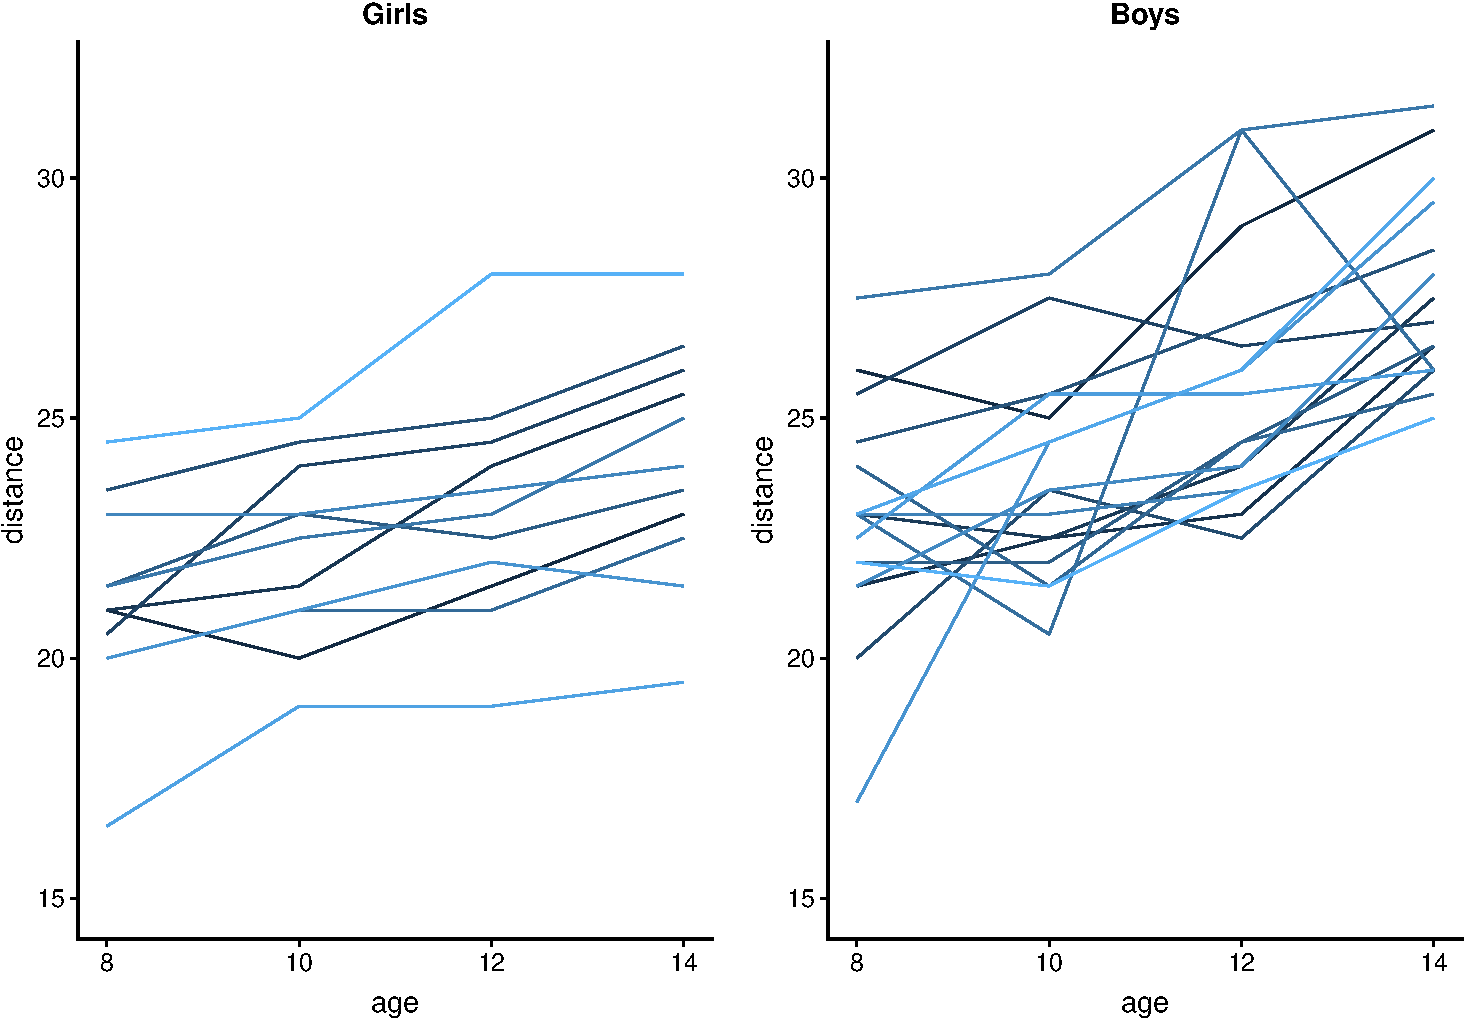
\includegraphics{Chapter5CodePart1_files/figure-beamer/plot1-1.pdf}

\end{frame}

\begin{frame}{Plots show:}

\begin{enumerate}
\def\labelenumi{\arabic{enumi}.}
\tightlist
\item
  variation among outcome at start (age 8 years),
\item
  increase over time, but not perfectly linear for subjects,
\item
  maybe one measurement error (boy that drops from age 12 to 14).
\end{enumerate}

\end{frame}

\begin{frame}[fragile]{Look at basic summaries with dplyr}

\begin{Shaded}
\begin{Highlighting}[]
\CommentTok{# get number of obs per person and mean}
\NormalTok{sum_dat=}\KeywordTok{group_by}\NormalTok{(dat,child) }\OperatorTok\StringTok{ }\KeywordTok{summarise}\NormalTok{(}\DataTypeTok{mean=}\KeywordTok{mean}\NormalTok{(distance),}\DataTypeTok{n=}\KeywordTok{n}\NormalTok{(),}\DataTypeTok{gender=}\KeywordTok{first}\NormalTok{(gender))}
\KeywordTok{table}\NormalTok{(sum_dat}\OperatorTok{$}\NormalTok{gender)}
\end{Highlighting}
\end{Shaded}

\begin{verbatim}
## 
##  0  1 
## 11 16
\end{verbatim}

\end{frame}

\begin{frame}{Linear model of distance by age and gender}

\begin{itemize}
\tightlist
\item
  \(Y_{ij}\) distance of the jth measurement on the ith child,
\item
  \(X_{ij1}\) is the age of ith child, jth measurement,
\item
  \(X_{ij2}\) is the gender of ith child, jth measurement (1 is male, 0
  is female) - same for all \(j =1,...,4\) measurements.
\end{itemize}

\[ Y_{ij} = \beta_0 +\beta_1 X_{ij1}+\beta_2 X_{ij2} + \beta_3 X_{ij1}X_{ij2}+e_{ij}, E(e_{ij}|X_{ij})=0 \]

\end{frame}

\begin{frame}{Oridinary Least Squares}

\begin{itemize}
\tightlist
\item
  The name is based on the objective function, that is:
\end{itemize}

\[ \hat{\beta} \equiv argmin_{\beta} \sum_{i=1}^n \sum_{j=1}^4(Y_{ij}-[\beta_0 +\beta_1 X_{ij1}+\beta_2 X_{ij2} + \beta_3 X_{ij1}X_{ij2}]) ^2 \]

\begin{itemize}
\item
  So, it minimizes the mean-squared error, or the squared residuals
  \(r_{ij} \equiv Y_{ij}-[\beta_0 +\beta_1 X_{ij1}+\beta_2 X_{ij2} + \beta_3 X_{ij1}X_{ij2}]\)
\item
  Can be motivated in two ways

  \begin{itemize}
  \tightlist
  \item
    Maximum likelihood estimation by assuming, for example,
    \(e_{ij} \sim N(0,\sigma_e)\)
  \item
    As the procedures that minimizes the squared residuals, regardless
    of distribution of \(e_{ij}\)
  \end{itemize}
\end{itemize}

\end{frame}

\begin{frame}{MLE Justification}

\begin{itemize}
\tightlist
\item
  Assume independent and identically distributed
  \(e_{ij} \sim N(0,\sigma_e)\) (so for now, observations are
  independent regardless if they are made on same child).
\item
  The likelihood is defined as simply the probability of the observed
  data. In this case, we can define the likelihood of one observation
  as: \(P(Y_{ij}\mid X_{ij1}, X_{ij2})P(X_{ij1},X_{ij2})\)\\
\item
  However, we can ignore the 2nd term (our parameters of interest are
  not a function of the distribution of \(P(X_{ij1},X_{ij2})\)).
\end{itemize}

\end{frame}

\begin{frame}{MLE , cont.}

\begin{itemize}
\tightlist
\item
  The likelihood of all the observations is (if they are all
  independent) the probability of each observation multiplied together
  (e.g., \(P(A \& B)=P(A)P(B)\) if independent).
  \[ = P(Y_{11} \mid X_{111},X_{112}) P(Y_{12} \mid X_{121},X_{122}) \]
  \[ \cdots P(Y_{m3} \mid X_{m31},X_{m32}) P(Y_{m4} \mid X_{m41},X_{m42})\]
\end{itemize}

\[ = \prod_{i=1}^m \prod_{j=1}^4 P(Y_{ij}\mid X_{ij1}, X_{ij2})\]

\begin{itemize}
\tightlist
\item
  If we assume a normal distribution for the \(e_{ij}\), then the
  distribution of \(Y_{ij} \mid X_{ij1}, X_{ij2}\) is also normal, since
  the rest of the linear equation is fixed when the X's are fixed.
\end{itemize}

\end{frame}

\begin{frame}{Distribution of \(Y|X\) in this model is distribution of
\(e\).}

\begin{itemize}
\tightlist
\item
  Note that
  \(e_{ij} = Y_{ij}-[\beta_0 +\beta_1 X_{ij1}+\beta_2 X_{ij2} + \beta_3 X_{ij1}X_{ij2}]\),
  so that
  \[P(Y_{ij} \mid X_{ij1}, X_{ij2}) = P(e_{ij} \mid X_{ij1}, X_{ij2}) \]
  \[= P(Y_{ij}-[\beta_0 +\beta_1 X_{ij1}+\beta_2 X_{ij2} + \beta_3 X_{ij1}X_{ij2}]) \]
  \[ = \phi \Big(\frac{Y_{ij}-[\beta_0 +\beta_1 X_{ij1}+\beta_2 X_{ij2} + \beta_3 X_{ij1}X_{ij2}]}{\sigma_e}\Big)\],
  where \(\phi(x)\) represents the standard normal density
  \(=\frac{exp(x^2)}{\sqrt{2 \pi} }\).
\end{itemize}

\end{frame}

\begin{frame}{Likelihood function}

\begin{itemize}
\item
  Thus,for all the data the likelihood (as a function of \(\beta\)) is
  \[ L(\beta \mid data) = \prod_{i=1}^m \prod_{j=1}^4  \phi \Big(\frac{Y_{ij}-[\beta_0 +\beta_1 X_{ij1}+\beta_2 X_{ij2} + \beta_3 X_{ij1}X_{ij2}]}{\sigma_e}\Big)\]
\item
  For several reasons, the log of this function is maximized (the
  maximum of the function, w.r.t. \(\beta\) or its log is the same)
\end{itemize}

\[ l(\beta \mid data) = \sum_{i=1}^m \sum_{j=1}^4 log \Big[ \phi \Big(\frac{Y_{ij}-[\beta_0 +\beta_1 X_{ij1}+\beta_2 X_{ij2} + \beta_3 X_{ij1}X_{ij2}]}{\sigma_e}\Big) \Big] \]

\begin{itemize}
\tightlist
\item
  taking the log of the \(\phi\) function is
  \[ log \Bigg( \frac{exp \Big(- \frac{\{Y_{ij}-[\beta_0 +\beta_1 X_{ij1}+\beta_2 X_{ij2} + 
  \beta_3 X_{ij1}X_{ij2}] \}^2}{2\sigma^2_e}\Big)}{\sqrt{2 \pi \sigma^2_e} } \Bigg) \]
  \[ = -\Big(  \frac{ \{Y_{ij}-[\beta_0 +\beta_1 X_{ij1}+\beta_2 X_{ij2} + \beta_3 X_{ij1}X_{ij2}]\}^2}{2 \sigma^2_e}\Big) - 1/2 * log(2 \pi \sigma^2_e)\]
\end{itemize}

\end{frame}

\begin{frame}{Maximizing likelihood}

\begin{itemize}
\item
  So, maximizing the log-likelihood is the same as minimizing the
  \[MSE(\beta) \equiv \frac{1}{N} \sum_{i=1}^n \sum_{j=1}^4(Y_{ij}-[\beta_0 +\beta_1 X_{ij1}+\beta_2 X_{ij2} + \beta_3 X_{ij1}X_{ij2}]) ^2 \].
\item
  Thus one can define OLS as
\end{itemize}

\[ \hat{\beta} \equiv argmin_{\beta} MSE(\beta) \]

\end{frame}

\begin{frame}{Properties of MLE}

\begin{itemize}
\tightlist
\item
  If you believe a particular parametric model for the data-generating
  distn, then: MLE's have \textbf{invariance property}:

  \begin{itemize}
  \tightlist
  \item
    if \(\hat{\beta}_n\) is the MLE, then any function of them is the
    MLE esitmate, \(h(\hat{\beta}_n)\) is the MLE of
    \(h(\beta_{true})\).
  \item
    e.g., if \(\hat{\beta}_n\) is MLE, then \(e^{\hat{\beta}_n}\) is
    also an MLE.
  \end{itemize}
\item
  \textbf{Asymptotically unbiased} (consistent), that is for any
  \[\epsilon > 0, lim_{n \rightarrow \infty} P(|\hat{\beta}_n-\beta_{true}|>\epsilon) \rightarrow 0. \]
\item
  \textbf{Asymptotically linear}: \(\hat{\beta}_n \approx \beta_{true}\)
  plus i.i.d. terms with mean 0.
\item
  \textbf{Asymptotically efficient}: if \(\tilde{\beta_n}\) is a
  competing estimator in same model, then
  \[lim_{n \rightarrow \infty} \Big[ \frac{var(\hat{\beta_n})}{var(\tilde{\beta_n})} \Big] \le 1 \]
\end{itemize}

\end{frame}

\begin{frame}{Motivating OLS as estimating equation}

\begin{itemize}
\tightlist
\item
  OLS also can be motivated without knowing the likelihood of the data
  (e.g., without asserting that \(e \sim N(0,\sigma_e)\)).
\item
  It turns out that the estimating equation is consistent for \(\beta\)
  regardless of the distribution of \(e \mid X_{ij}\).
\item
  In general, an estimating equation results in a consistent estimator
  of \(\beta_{true}\) if \(E_{\beta_{true}}g(O_i,\beta_{true})=0\),
  where \(g(,)\) is an estimating equation, and \(O_i\) is the data on
  one statistical unit, so in our case,
  \(O_i=(Y_{ij},\vec{X}_{ij},j=1,...,4)\).\\
\item
  These leads to an estimator by solving
  \(\frac{1}{m} \sum_{i = 1}^m g(O_i,\beta) = 0\).
\end{itemize}

\end{frame}

\begin{frame}{OLS as Solution to minimizing MSE}

\begin{itemize}
\tightlist
\item
  One has a function that one is trying to minimize w.r.t. \(\beta\),
  i.e., \(argmin_{\beta} MSE(\beta)\)
\item
  Let's take a simple linear model for now with one predictor:
  \(Y_{ij} = \beta_0+\beta_1 X_{ij}+e\), so minimizing the MSE is same
  as minimizing:
\item
  Minimizing the function specifically in this case, is minimizing
  \[MSE(\beta) = \sum_{i=1}^n \sum_{j=1}^4(Y_{ij}-[\beta_0 +\beta_1 X_{ij}]) ^2 \].
\end{itemize}

\end{frame}

\begin{frame}{Minimizing function}

\begin{itemize}
\tightlist
\item
  How does one minimize functions?

  \begin{itemize}
  \tightlist
  \item
    Try an exhaustive grid over all possible values of the parameters
    \(\beta=(\beta_0,\beta_1)\) and find the combo that has smalles
    \(MSE(\beta)\)
  \item
    Find the solution analytically using calculus.
  \end{itemize}
\item
  One can solve a set of two differential equations in this case, so:
  \[ \frac{\partial MSE(\beta)}{\partial \beta_0} = 0 \] and
  \[ \frac{\partial MSE(\beta)}{\partial \beta_1} = 0 \]
\item
  Solve for \((\beta_0, \beta_1)\).
\item
  Show on board.
\item
  In this case, one gets the following general solution (in matrix
  form):
  \[\hat{\vec{\beta_n}} = \boldsymbol{(X X^T) }^{-1} \boldsymbol{X}^T \vec{Y}\]
\end{itemize}

\end{frame}

\begin{frame}{Is this a consistent estimator?}

\begin{itemize}
\tightlist
\item
  We now from theory, if it's the MLE, it is a consistent estimator (see
  above).
\item
  However, is it more generally consistent than that?
\item
  Just have to plug and chug to see what is the expected value of this
  estimator, \(E(\hat{\beta_n})\) and whether it is equal to the true
  \(\beta_{true}\).\\
\item
  This one is ``easy'':
  \[E(\hat{\beta_n}\mid \boldsymbol{X})=E\{ \boldsymbol{(X X^T) }^{-1} \boldsymbol{X}^T \vec{Y} \mid \boldsymbol{X} \} \]
  \[=
  \boldsymbol{(X X^T) }^{-1} \boldsymbol{X}^T E(\vec{Y} \mid \boldsymbol{X}) \]
  \[ = \boldsymbol{(X X^T) }^{-1} \boldsymbol{X}^T  \boldsymbol{X} \vec{\beta}_{true} = \vec{\beta}_{true}\]
\end{itemize}

\end{frame}

\begin{frame}{What about impact of repeated measures (dependent data)?}

\begin{itemize}
\tightlist
\item
  The dependence among observations on same subject does not impact the
  ``proof''

  \begin{itemize}
  \tightlist
  \item
    This is because expectation of sums is sum of expectations, e.g.,
    \(E(\sum_{i=1}^m \sum_{j=1}^{n_i} Y_{ij}) = \sum_{i=1}^m \sum_{j=1}^{n_i} E(Y_{ij})\)
  \item
    Note, this is NOT generally true for variances of sum - that the
    variance of sum is only equal to sum of variances if the random
    variables are independent.
  \end{itemize}
\item
  Thus, it looks like ignoring the dependence does not necessarily cause
  bias in estimation of the coefficients (generally true, but gets
  complicated in more complicated setting with unequal numbers of
  measurements per unit, and if the linear model is misspecified).
\end{itemize}

\end{frame}

\begin{frame}{Variance of coefficient estimates from OLS fit
(\(var(\hat{\beta}_n)\)).}

\begin{itemize}
\tightlist
\item
  Note that \(\hat{\beta}_n = (\hat{\beta}_{0,n}, \hat{\beta}_{1,n})\)
  is a vector the variance of a vector implies the variance-covariance
  matrix, or a matrix with the variance of all parameter estimates and
  all pairwise covariances.\\
\item
  So, when we say we want the \(var(\hat{\beta}_n)\), which we sometimes
  represent as \(V_{\hat{\beta}_n}\),it means the estimate of each
  component of the following in our simple linear model case
  (\(Y_{ij} = \beta_0+\beta_1 X_{ij}+e\)), so \[
  V_{\hat{\beta}_n} = 
  \begin{bmatrix}
  var(\hat{\beta}_{0,n})        & cov (\hat{\beta}_{0,n},\hat{\beta}_{1,n}) \\
  cov (\hat{\beta}_{0,n},\hat{\beta}_{1,n})   & var(\hat{\beta}_{1,n})
  \end{bmatrix}
  \]
\item
  We want to derive an estimate of this (since we never know it) so \[
  \hat{V}_{\hat{\beta}_n} = 
  \begin{bmatrix}
  \hat{var}(\hat{\beta}_{0,n})        & \hat{cov} (\hat{\beta}_{0,n},\hat{\beta}_{1,n}) \\
  \hat{cov} (\hat{\beta}_{0,n},\hat{\beta}_{1,n})   & \hat{var}(\hat{\beta}_{1,n})
  \end{bmatrix}
  \]
\end{itemize}

\end{frame}

\begin{frame}{Standard errors}

\begin{itemize}
\tightlist
\item
  Note that the standard errors reported in regression outputs are based
  upon this estimated matrix, e.g.,
  \(SE(\hat{\beta}_{1,n}) = \sqrt{\hat{var}(\hat{\beta}_{1,n})}\).
\item
  If we ever want to report an estimated parameter that involves more
  than one coefficient estimate, then we also need the covariance terms
  (though we can have procedures that automate this process).
\end{itemize}

\end{frame}

\begin{frame}{Review some rules of expectation and variance for random
variables and vectors.}

\begin{itemize}
\tightlist
\item
  Expectation of sum is sum of expectations
  \[E(\sum_{i=1}^m \sum_{j=1}^{n_i} Y_{ij}) = \sum_{i=1}^m \sum_{j=1}^{n_i} E(Y_{ij})\]
\item
  Expectation of constant times random variable (vector) is constant
  times expectation of random variable (vector) \[ E(AY) = AE(Y) \]
  \[ E(\vec{A}^T \vec{Y}) = A^T E(\vec{Y}) \]
\item
  Variance of constant times random variable is constant squared times
  variance of random variable \[ var(AY) = A^2 var(Y)\]
  \[ var(\vec{A}^T \vec{Y}) = \vec{A}^T V_{\vec{Y}} \vec{A}\]
\end{itemize}

\end{frame}

\begin{frame}{Using rules to get \(var(\hat{\beta}_n)\)}

\begin{itemize}
\tightlist
\item
  Get
  \[var(\hat{\beta_n}\mid \boldsymbol{X})=var\{ \boldsymbol{(X^T X ) }^{-1} \boldsymbol{X}^T \vec{Y} \mid \boldsymbol{X} \} \].
\item
  Not that this is same situation as the matrix version of the variance
  of a constant times a random variable
\item
  In this case, matrix of constants
  (\(\boldsymbol{(X^T X ) }^{-1} \boldsymbol{X}^T\)) times a random
  vector (\(\vec{Y}\)).
\item
  Using the rule above, this means that:
  \[var\{ \boldsymbol{(X^T X ) }^{-1} \boldsymbol{X}^T \vec{Y} \mid \boldsymbol{X} \} = \boldsymbol{(X^T X ) }^{-1} \boldsymbol{X}^T V_{\vec{Y}}[\boldsymbol{(X^T X ) }^{-1} \boldsymbol{X}^T]^T\]
\item
  Using rules of matrix transformation, one gets:
  \[ var(\hat{\beta_n}\mid \boldsymbol{X})= \boldsymbol{(X^T X ) }^{-1} \boldsymbol{X}^T V_{\vec{Y}} \boldsymbol{X} \boldsymbol{(X^T X ) }^{-1} \]
\item
  The term ``sandwich estimator'' of the variance comes from this form
  where the sandwich filling is the variance-covariance matrix of
  \(\vec{Y} \mid \boldsymbol{X}\), or \(V_{\vec{Y}}\) and the bread is
  the \(\boldsymbol{(X^T X ) }^{-1} \boldsymbol{X}^T\).
\end{itemize}

\end{frame}

\begin{frame}{Estimating \(var(\hat{\beta_n}\mid \boldsymbol{X})\)}

\begin{itemize}
\tightlist
\item
  All the matrices \(\boldsymbol{X}\) are known (we are conditioning on
  them)
\item
  The only unknown matrix is \(V_{\vec{Y}}\), or the variance covariance
  of the outcomes.
\item
  Thus, we have to estimate it in order to fill in the unknown
  components of it.
\item
  This is where assumptions about the ``form'' of the
  variance-covariance (VC) matrix, that is assumptions of how the
  observations are potentially dependent, have an impact.
\end{itemize}

\end{frame}

\begin{frame}{a}

\includegraphics[page=2,width=5in]{Chapter5AddSlides1.pdf}

\end{frame}

\begin{frame}{b}

\includegraphics[page=3,width=5in]{Chapter5AddSlides1.pdf}

\end{frame}

\begin{frame}{c}

\includegraphics[page=4,width=4.5in]{Chapter5AddSlides1.pdf}

\end{frame}

\begin{frame}{d}

\includegraphics[page=5,width=4.5in]{Chapter5AddSlides1.pdf}

\end{frame}

\begin{frame}{e}

\includegraphics[page=6,width=4.5in]{Chapter5AddSlides1.pdf}

\end{frame}

\begin{frame}{f}

\includegraphics[page=7,width=4.5in]{Chapter5AddSlides1.pdf}

\end{frame}

\begin{frame}{g}

\includegraphics[page=8,width=4.5in]{Chapter5AddSlides1.pdf}

\end{frame}

\begin{frame}{h}

\includegraphics[page=9,width=4.5in]{Chapter5AddSlides1.pdf}

\end{frame}

\begin{frame}{i}

\includegraphics[page=10,width=4.5in]{Chapter5AddSlides1.pdf}

\end{frame}

\begin{frame}{j}

\includegraphics[page=11,width=5.5in]{Chapter5AddSlides1.pdf}

\end{frame}

\begin{frame}{k}

\includegraphics[page=12,width=5.5in]{Chapter5AddSlides1.pdf}

\end{frame}

\begin{frame}{l}

\includegraphics[page=13,width=5.5in]{Chapter5AddSlides1.pdf}

\end{frame}

\begin{frame}{m}

\includegraphics[page=14,width=7in]{Chapter5AddSlides1.pdf}

\end{frame}

\begin{frame}{n}

\includegraphics[page=15,width=5.5in]{Chapter5AddSlides1.pdf}

\end{frame}

\begin{frame}{Estimate linear model for dental data}

\begin{itemize}
\tightlist
\item
  Again, the model we wanted to estimate is:
\end{itemize}

\[ E(Y_{ij} \mid \vec{X}_{ij}) = \beta_0 +\beta_1 X_{ij1}+\beta_2 X_{ij2} + \beta_3 X_{ij1}X_{ij2} \]

\end{frame}

\begin{frame}[fragile]{Use simple OLS}

\tiny

\begin{Shaded}
\begin{Highlighting}[]
\CommentTok{# First, make interaction term}
\KeywordTok{library}\NormalTok{(RCurl)}
\NormalTok{dat =}\StringTok{ }\NormalTok{dat }\OperatorTok\StringTok{ }\KeywordTok{mutate}\NormalTok{(}\DataTypeTok{inter=}\NormalTok{gender}\OperatorTok{*}\NormalTok{age)}
\NormalTok{ols_fit =}\StringTok{ }\KeywordTok{lm}\NormalTok{(distance }\OperatorTok{~}\StringTok{ }\NormalTok{gender}\OperatorTok{+}\NormalTok{age}\OperatorTok{+}\NormalTok{inter, }\DataTypeTok{data=}\NormalTok{dat)}
\KeywordTok{summary}\NormalTok{(ols_fit)}
\end{Highlighting}
\end{Shaded}

\begin{verbatim}
## 
## Call:
## lm(formula = distance ~ gender + age + inter, data = dat)
## 
## Residuals:
##     Min      1Q  Median      3Q     Max 
## -5.6156 -1.3219 -0.1682  1.3299  5.2469 
## 
## Coefficients:
##             Estimate Std. Error t value Pr(>|t|)    
## (Intercept)  17.3727     1.7080  10.171  < 2e-16 ***
## gender       -1.0321     2.2188  -0.465  0.64279    
## age           0.4795     0.1522   3.152  0.00212 ** 
## inter         0.3048     0.1977   1.542  0.12608    
## ---
## Signif. codes:  0 '***' 0.001 '**' 0.01 '*' 0.05 '.' 0.1 ' ' 1
## 
## Residual standard error: 2.257 on 104 degrees of freedom
## Multiple R-squared:  0.4227, Adjusted R-squared:  0.4061 
## F-statistic: 25.39 on 3 and 104 DF,  p-value: 2.108e-12
\end{verbatim}

\end{frame}

\begin{frame}{Output to reporting}

\begin{itemize}
\tightlist
\item
  Because of the interaction term, one can not interpret the individual
  coefficients as easily as a model with only main terms.
\item
  The first thing is to decide what is a good measure of association.
\item
  First lets take age:

  \begin{itemize}
  \tightlist
  \item
    must choose a change of age: lets take 6 years
  \item
    For now, we will Assume that gender is set to some fixed value,
    \(g\).
  \end{itemize}
\end{itemize}

\[ E(Y_{ij} \mid X_{ij1}=age+6,X_{ij2}=g) -  E(Y_{ij} \mid X_{ij1}=age,X_{ij2}=g) \]

\[ = \beta_0 +\beta_1 (age+6)+\beta_2 g + \beta_3 (age+6)*g \]

\[ - [\beta_0 +\beta_1 age+\beta_2 g + \beta_3 age*g] \]

\[ = 6*\beta_1 + 6*g*\beta_3\]

\end{frame}

\begin{frame}{Getting estimates of linear combination of coefficients}

\begin{itemize}
\tightlist
\item
  The previous slide shows that, for females:
\end{itemize}

\[ E(Y_{ij} \mid X_{ij1}=age+6,X_{ij2}=1) -  E(Y_{ij} \mid X_{ij1}=age,X_{ij2}=1) \]
\[ =  6*\beta_1 + 6*\beta_3\] - Thus, we want to get an estimate of (and
standard error for): \(6*\hat{\beta}_1 + 6*\hat{\beta}_3\).

\begin{itemize}
\tightlist
\item
  We've already done this based on user-written function, but this time
  we'll use an exsiting function in the \textbf{multcomp} package.
\end{itemize}

\end{frame}

\begin{frame}[fragile]{Get estimates and inference for linear
combination of coefficients using the ``naive'' inference returned by
the OLS procedure.}

\tiny

\begin{Shaded}
\begin{Highlighting}[]
\NormalTok{## Note how the algebra is entered into function}
\NormalTok{### For boys}
\NormalTok{lin.boys=}\KeywordTok{glht}\NormalTok{(ols_fit, }\DataTypeTok{linfct =} \KeywordTok{c}\NormalTok{(}\StringTok{"6*age +6*inter=0"}\NormalTok{))}
\CommentTok{#summary(lin.boys)}
\KeywordTok{confint}\NormalTok{(lin.boys)  }
\end{Highlighting}
\end{Shaded}

\begin{verbatim}
## 
##   Simultaneous Confidence Intervals
## 
## Fit: lm(formula = distance ~ gender + age + inter, data = dat)
## 
## Quantile = 1.983
## 95% family-wise confidence level
##  
## 
## Linear Hypotheses:
##                          Estimate lwr    upr   
## 6 * age + 6 * inter == 0 4.7063   3.2051 6.2074
\end{verbatim}

\end{frame}

\begin{frame}[fragile]{Repeat for girls}

In this case,
\[ E(Y_{ij} \mid X_{ij1}=age+6,X_{ij2}=0) -  E(Y_{ij} \mid X_{ij1}=age,X_{ij2}=0) \]
\[ =  6*\beta_1\]

\tiny

\begin{Shaded}
\begin{Highlighting}[]
\NormalTok{lin.girls=}\KeywordTok{glht}\NormalTok{(ols_fit, }\DataTypeTok{linfct =} \KeywordTok{c}\NormalTok{(}\StringTok{"6*age=0"}\NormalTok{))}
\CommentTok{#summary(lin.girls)}
\KeywordTok{confint}\NormalTok{(lin.girls)  }
\end{Highlighting}
\end{Shaded}

\begin{verbatim}
## 
##   Simultaneous Confidence Intervals
## 
## Fit: lm(formula = distance ~ gender + age + inter, data = dat)
## 
## Quantile = 1.983
## 95% family-wise confidence level
##  
## 
## Linear Hypotheses:
##              Estimate lwr    upr   
## 6 * age == 0 2.8773   1.0668 4.6877
\end{verbatim}

The results suggest that the mean change in the distance for boys is
4.76 (95\% 3.20-6.21) and that for girls is 2.88 (95\% 1.07-4.69).

\end{frame}

\begin{frame}{Robust estimation of SE's}

\begin{itemize}
\item
  Here, we are beginning the meat of the course, getting inference that
  can account for the potential repeated measures structure.
\item
  We will explore many methods that can do this with varying numbers of
  assumptions
\item
  Here we start with some of the methods are meant to give
  \textbf{nonparametric inference} for any general linear model
  estimators.
\end{itemize}

\end{frame}

\begin{frame}[fragile]{Inference for sandwich estimator}

\tiny

\begin{Shaded}
\begin{Highlighting}[]
\CommentTok{# Read in user written function using lmtest and }
\CommentTok{# sandwich packages that return both information }
\CommentTok{# on coefficients and estimates of linear}
\CommentTok{# combination of coefficients using}
\CommentTok{# clustered/robust variance estimates}
\KeywordTok{source}\NormalTok{(}\StringTok{"clx.R"}\NormalTok{)}
\KeywordTok{source}\NormalTok{(}\StringTok{"clx_lincom.R"}\NormalTok{)}

\KeywordTok{clx}\NormalTok{(ols_fit, }\DecValTok{1}\NormalTok{, dat}\OperatorTok{$}\NormalTok{child)}
\end{Highlighting}
\end{Shaded}

\begin{verbatim}
## 
## t test of coefficients:
## 
##              Estimate Std. Error t value  Pr(>|t|)    
## (Intercept) 17.372727   0.749604 23.1759 < 2.2e-16 ***
## gender      -1.032102   1.424137 -0.7247   0.47025    
## age          0.479545   0.065257  7.3486 4.712e-11 ***
## inter        0.304830   0.120799  2.5234   0.01313 *  
## ---
## Signif. codes:  0 '***' 0.001 '**' 0.01 '*' 0.05 '.' 0.1 ' ' 1
\end{verbatim}

\begin{Shaded}
\begin{Highlighting}[]
\CommentTok{# Robust estimate for change in mean}
\CommentTok{# for 6 year increase in age for}
\CommentTok{# boys}
\KeywordTok{clx.lincom}\NormalTok{(ols_fit, }\DecValTok{1}\NormalTok{,dat}\OperatorTok{$}\NormalTok{child, }\KeywordTok{c}\NormalTok{(}\DecValTok{0}\NormalTok{,}\DecValTok{0}\NormalTok{,}\DecValTok{6}\NormalTok{,}\DecValTok{6}\NormalTok{))}
\end{Highlighting}
\end{Shaded}

\begin{verbatim}
##      Est      CI                pvalue  
## [1,] "4.7063" "3.5108 - 5.9017" "0.0000"
\end{verbatim}

\end{frame}

\begin{frame}{Comparison of results}

\begin{itemize}
\tightlist
\item
  If one looks at the age coefficient, one can see that the robust SE is
  much smaller than the naive one returned by standard OLS: 0.065 vs
  0.152.\\
\item
  We can also compare the results of the estimate of\\
  \[ =  6*\beta_1 + 6*\beta_3\] and we see the CI based upon the robust
  estimates that account for dependence is 3.511-5.911 versus
  3.205-6.207, so for this parameter, the CI gets bigger when the SE is
  estimated correctly.
\end{itemize}

\end{frame}

\begin{frame}{Conclusions}

\begin{itemize}
\tightlist
\item
  One can motivate standard ordinary least squares estimation by either
  maximum likelihood estimation or estimating equation.
\item
  Ignoring the repeated measures structures does not affect the
  biasedness of the OLS estimates of the coefficients.
\item
  However, the standard errors returned assuming independence are
  biased.
\item
  We can fix these by procedures that assume nothing about the
  covariance of observations within the same unit.
\end{itemize}

\end{frame}

\end{document}
